\documentclass{ximeraXloud}

\title{Parent Functions}
\begin{document}
\begin{abstract}
    This is practice for Parent Functions
\end{abstract}
\maketitle


%% Necessary code to graph in the following sections:
\pgfplotsset{my style/.append style={axis x line=middle, axis y line=middle, xlabel={$x$}, ylabel={$y$} }}

\begin{problem}
    Consider the following graph:
    \begin{center}
        \begin{tikzpicture}
            \begin{axis}[
                axis x line=middle, 
                axis y line=middle, 
                xlabel={$x$}, 
                ylabel={$y$}, 
                xtick={-4,-2,...,10}, 
                ytick={-6,-4,...,10},
                xmin=-3, 
                xmax=10, 
                ymin=-5, 
                ymax=10
                ]
                \addplot[<->,domain=-2.9:9, samples=300]{-2*ln(x+3) + 4};
            \end{axis}
        \end{tikzpicture}
    \end{center}
    
    What is the best parent function for the graph?
    
    \begin{multipleChoice}
        \choice{$f(x)=x$}
        \choice{$f(x)=x^2$}
        \choice{$f(x)=x^3$}
        \choice{$f(x)=\sqrt{x}$}
        \choice{$f(x)=e^x$}
        \choice[correct]{$f(x)=\ln(x)$}
        \choice{$f(x)=|x|$}
    \end{multipleChoice}
    
    
\end{problem}
        
        
\begin{problem}
    Consider the following graph:
    \begin{center}
        \begin{tikzpicture}
            \begin{axis}[
                axis x line=middle, 
                axis y line=middle, 
                xlabel={$x$}, 
                ylabel={$y$}, 
                xtick={-3,-2,...,5},
                ytick={-80,-60,...,100},
                xmin=-3, 
                xmax=5, 
                ymin=-85, 
                ymax=105
                ]
                \addplot[<->,domain=-2:4, samples=300]{3*(x-1)*(x-1)*(x-1) + 1};
            \end{axis}
        \end{tikzpicture}
    \end{center}
    
    What is the best parent function for the graph?
    
    \begin{multipleChoice}
        \choice{$f(x)=x$}
        \choice{$f(x)=x^2$}
        \choice[correct]{$f(x)=x^3$}
        \choice{$f(x)=\sqrt{x}$}
        \choice{$f(x)=e^x$}
        \choice{$f(x)=\ln(x)$}
        \choice{$f(x)=|x|$}
    \end{multipleChoice}
    
    
\end{problem}
        
       
        
\begin{problem}
    Consider the following graph:
    \begin{center}
        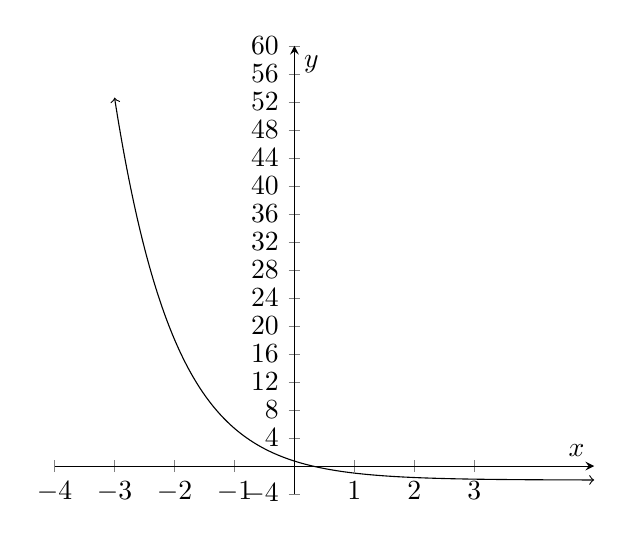
\begin{tikzpicture}
            \begin{axis}[
                axis x line=middle, 
                axis y line=middle, 
                xlabel={$x$}, 
                ylabel={$y$}, 
                xtick={-5,-4,...,3},
                ytick={-4,0,...,60},
                xmin=-4, 
                xmax=5, 
                ymin=-4, 
                ymax=60
                ]
                \addplot[<->,domain=-3:5, samples=300]{e^(-x+1) -2};
            \end{axis}
        \end{tikzpicture}
    \end{center}
    
    What is the best parent function for the graph?
    
    \begin{multipleChoice}
        \choice{$f(x)=x$}
        \choice{$f(x)=x^2$}
        \choice{$f(x)=x^3$}
        \choice{$f(x)=\sqrt{x}$}
        \choice[correct]{$f(x)=e^x$}
        \choice{$f(x)=\ln(x)$}
        \choice{$f(x)=|x|$}
    \end{multipleChoice}
    
    
\end{problem}
        
        
        
\begin{problem}
    Consider the following graph:
    \begin{center}
        \begin{tikzpicture}
            \begin{axis}[
                axis x line=middle, 
                axis y line=middle, 
                xlabel={$x$}, 
                ylabel={$y$}, 
                xtick={-8,-6,...,2},
                ytick={0,1,...,4},
                xmin=-8, 
                xmax=2, 
                ymin=-1, 
                ymax=5
                ]
                \addplot[<-,domain=-7:-2, samples=300]{sqrt(-x-2)+1};
            \end{axis}
        \end{tikzpicture}
    \end{center}
    
    What is the best parent function for the graph?
    
    \begin{multipleChoice}
        \choice{$f(x)=x$}
        \choice{$f(x)=x^2$}
        \choice{$f(x)=x^3$}
        \choice[correct]{$f(x)=\sqrt{x}$}
        \choice{$f(x)=e^x$}
        \choice{$f(x)=\ln(x)$}
        \choice{$f(x)=|x|$}
    \end{multipleChoice}
    
    
\end{problem}
        
        
                
        
\end{document}